
\lecture{Regression Analysis}{regression-analysis}
\section{Regression Analysis}

\title{Regression Analysis}
\subtitle{Analysis Of The Slope Of The Regression Line}

%\author{Kelly Black}
%\institute{Clarkson University}
\date{8 April 2015}

\begin{frame}
  \titlepage
\end{frame}

\begin{frame}
  \frametitle{Outline}
  \tableofcontents[hideothersubsections,sectionstyle=show/hide]
\end{frame}


\subsection{Clicker Quiz}


\begin{frame}
  \frametitle{Clicker Quiz}

    \iftoggle{clicker}{%

    \begin{columns}
      \column{.25\textwidth}

      \begin{tabular}{l|l}
        $X$ & $Y$ \\ \hline
        {\color{red}1} & {\color{blue}2} \\
        {\color{red}2} & {\color{blue}3}  \\
        {\color{red}3} & {\color{blue}3} \\
        {\color{red}4} & {\color{blue}5}  \\
        {\color{red}5} & {\color{blue}4}
      \end{tabular}

      \column{.75\textwidth}

      Is there a linear relationship between the two variables? (Use a
      95\% confidence level.)

      \begin{tabular}{l@{\hspace{3em}}l@{\hspace{3em}}l@{\hspace{3em}}l}
        A: Reject $H_0$  & B: Do not reject $H_0$
      \end{tabular}


      \begin{eqnarray*}
        {\color{red}\bar{x}} & = & {\color{red}3} \\
        {\color{blue}\bar{y}} & = & {\color{blue}3.4}
      \end{eqnarray*}

    \end{columns}

      \begin{eqnarray*}
        s_{xx} & = & \lp {\color{red}1-3}\rp^2 + \lp {\color{red}2 - 3} \rp^2 + \lp {\color{red}3 - 3} \rp^2 + 
                    \lp {\color{red}4 - 3} \rp^2 + \lp {\color{red}5 - 3} \rp^2 \\
        & = & 10, \\
        s_{yy} & = & \lp {\color{blue}2-3.4}\rp^2 + \lp {\color{blue}3 - 3.4} \rp^2 + \lp {\color{blue}3 - 3.4} \rp^2 + 
                    \lp {\color{blue}5 - 3.4} \rp^2 + \lp {\color{blue}4 - 3.4 }\rp^2 \\
        & = & 5.2, \\
        s_{xy} & = & \lp {\color{red}1-3}\rp\lp {\color{blue}2-3.4}\rp + \lp {\color{red}2 - 3} \rp\lp {\color{blue}3 - 3.4 }\rp + 
                    \lp {\color{red}3 - 3} \rp\lp {\color{blue}3 - 3.4 }\rp + \\
              &   & \lp {\color{red}4 - 3} \rp\lp {\color{blue}5 - 3.4} \rp + \lp {\color{red}5-4} \rp \lp {\color{blue}4-3.4} \rp \\
        & = & 6
      \end{eqnarray*}

    \vfill 




    }

\end{frame}




\subsection{Linear Regression}

\begin{frame}{Linear Regression}

  Given data can I find the ``best'' straight line
  \begin{eqnarray*}
    y & = & mx + b?
  \end{eqnarray*}


  \only<1>{\centerline{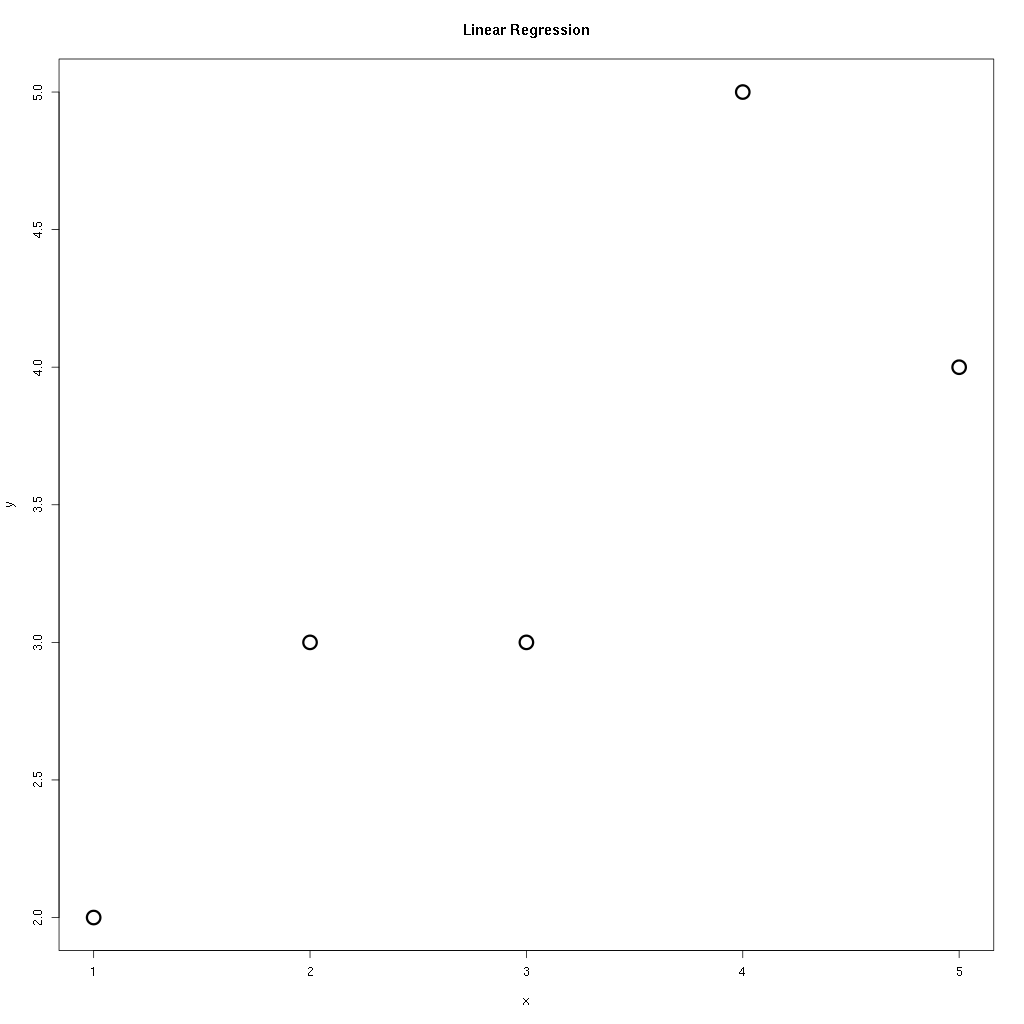
\includegraphics[width=4cm]{img/scatterLR-raw}}}
  \only<2>{\centerline{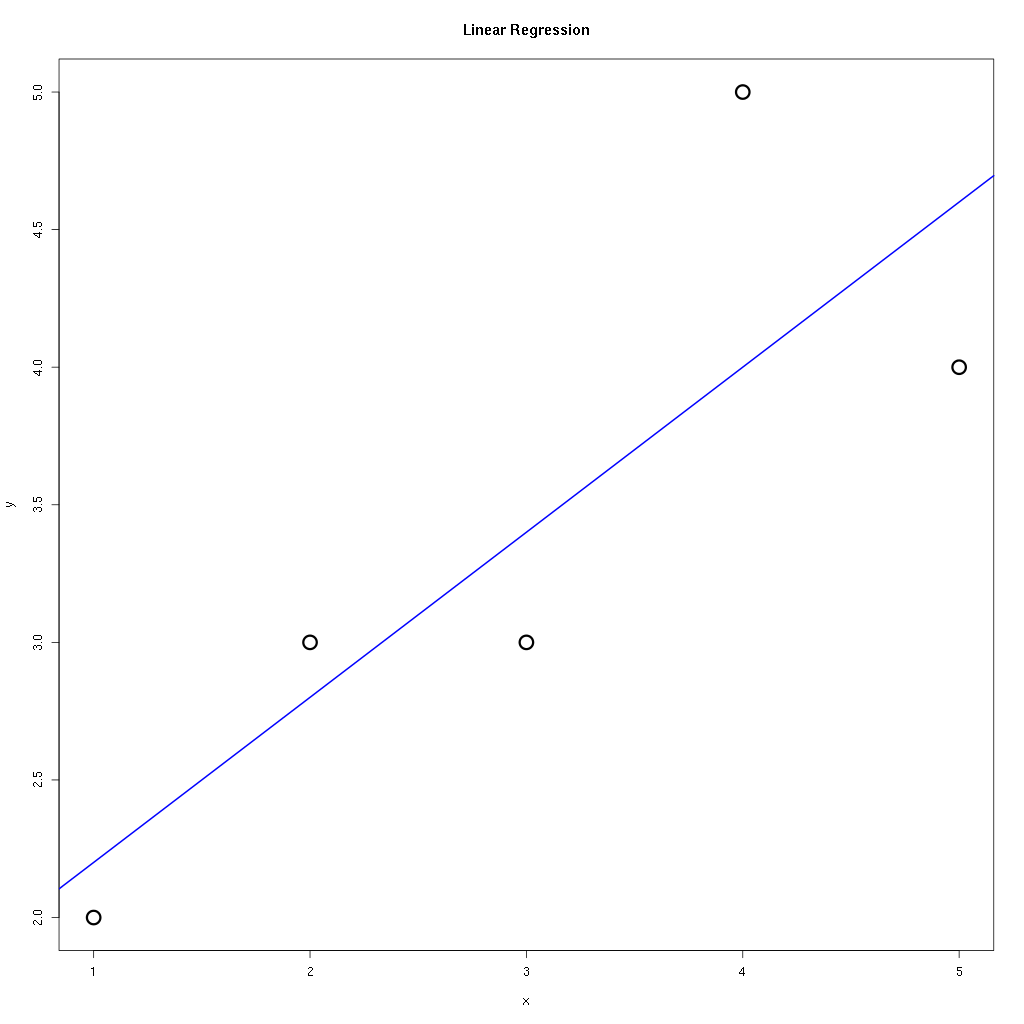
\includegraphics[width=4cm]{img/scatterLR-line}}}
  \only<3>{\centerline{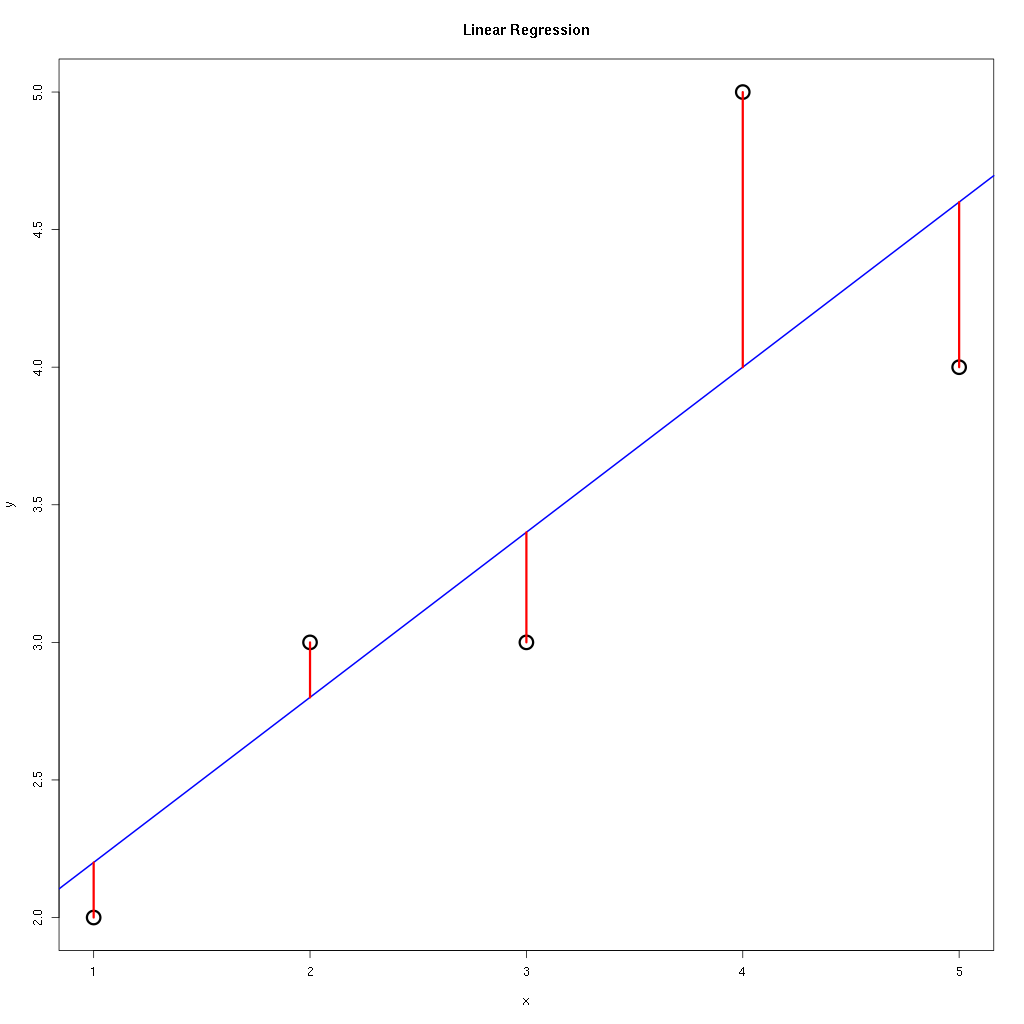
\includegraphics[width=4cm]{img/scatterLR-preResidual}}}
  \only<4->{%

    \centerline{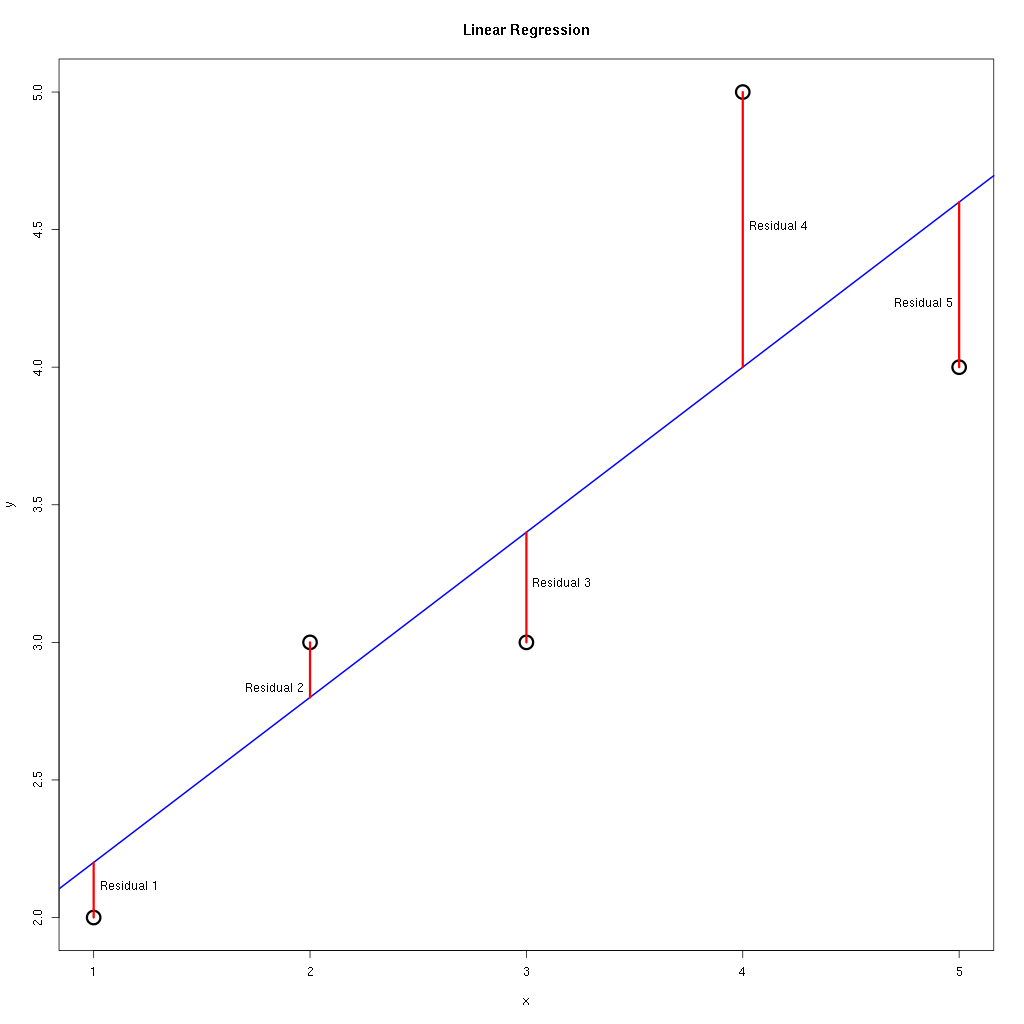
\includegraphics[width=4cm]{img/scatterLR-Residual}}
    
    \only<5->{%
      Goal: minimize
      \begin{eqnarray*}
        & & \lp\mathrm{residual~1}\rp^2 + \lp\mathrm{residual~2}\rp^2 + \\
        & & \lp\mathrm{residual~3}\rp^2 + \lp\mathrm{residual~4}\rp^2 + \lp\mathrm{residual~5}\rp^2 
      \end{eqnarray*}
    }

  }
  
\end{frame}

\begin{frame}
  \frametitle{Linear Regression}

    \begin{columns}
      \column{.65\textwidth}

      \centerline{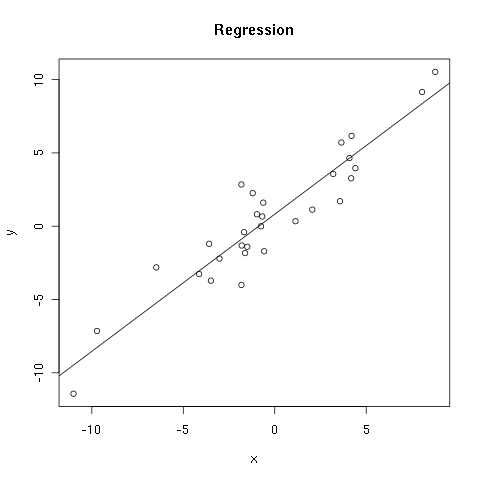
\includegraphics[width=6cm]{img/regressionGeneral}}

      \column{.35\textwidth}
      
      Our \textit{\color{red}approximation} for the best linear fit is
      \begin{eqnarray*}
        y & = & {\color{red}\hat{m}} x + {\color{red}\hat{b}}.
      \end{eqnarray*}
      where
      \begin{eqnarray*}
        \hat{m} & = & \frac{s_{xy}}{s_{xx}}, \\
        \hat{b} & = & \bar{y} - \hat{m} \bar{x}.
      \end{eqnarray*}

    \end{columns}

\end{frame}


\begin{frame}{The Residual}

  \begin{definition}
    The \textit{\color{red} predicted value} for $y$ at $x_i$ is
    \begin{eqnarray*}
      {\color{red}\hat{y}_i} & = & \hat{m} x_i + \hat{b}.
    \end{eqnarray*}

    The \textit{\color{red} residual} at $x_i$ is 
    \begin{eqnarray*}
      \mathrm{Residual}_i & = & y_i - \lp {\color{blue}\hat{m} x_i + \hat{b}} \rp, \\
      & = & y_i - {\color{blue}\hat{y}_i}.
    \end{eqnarray*}

  \end{definition}

  \only<2->
  {

    \begin{definition}
      The variance of the error is 
      \begin{eqnarray*}
        s^2_e & = & \frac{\lp y_1 - \hat{y}_1\rp^2 + \lp y_2 - \hat{y}_2\rp^2 + \cdots + \lp y_n - \hat{y}_n\rp^2 }{n-2}.
      \end{eqnarray*}
    \end{definition}

  }
  
\end{frame}

\begin{frame}{Example}

    \begin{columns}
      \column{.25\textwidth}

      \begin{tabular}{l|l}
        $X$ & $Y$ \\ \hline
        1 & 2 \\
        2 & 3  \\
        3 & 3 \\
        4 & 5  \\
        5 & 4
      \end{tabular}

      \column{.65\textwidth}

      \begin{eqnarray*}
        \bar{x} & = & 3 \\
        \bar{y} & = & 3.4 \\
        s_{xx} & = & 10, \\
        s_{yy} & = & 5.2, \\
        s_{xy} & = & 6
      \end{eqnarray*}

      \end{columns}

  \only<2->
  {

    \begin{eqnarray*}
      \hat{m} & = & \frac{s_{xy}}{s_{xx}}, \\
      & = & 0.6, \\
      \hat{b} & = & \bar{y} - \hat{m} \bar{x}, \\
      & = & 1.6
    \end{eqnarray*}

  }

  
\end{frame}



\begin{frame}{Example}

    \begin{columns}
      \column{.25\textwidth}

      \begin{tabular}{l|l}
        $X$ & $Y$ \\ \hline
        1 & 2 \\
        2 & 3  \\
        3 & 3 \\
        4 & 5  \\
        5 & 4
      \end{tabular}

      \column{.65\textwidth}

      \begin{eqnarray*}
        \bar{x} & = & 3 \\
        \bar{y} & = & 3.4 \\
        s_{xx} & = & 10, \\
        s_{yy} & = & 5.2, \\
        s_{xx} & = & 6, \\
        \hat{m} & = & 0.6, \\
        \hat{b} & = & 1.6
      \end{eqnarray*}

      \end{columns}

  \only<2->
  {

      \begin{tabular}{r|r<{\onslide<3->}|r<{\onslide<4->}|r<{\onslide}} % 
        $X$ & $Y$ & $\hat{Y}$ & Residual \\ \hline
        1 & 2 & 2.2 & -.2 \\
        2 & 3 & 2.8 &  .2 \\
        3 & 3 & 3.4 & -.4 \\
        4 & 5 & 4.0 & 1.0  \\
        5 & 4 & 4.6 & -.6
      \end{tabular}


  }

  
\end{frame}


\begin{frame}{Example}

  \begin{tabular}{r|r|r|r}
    $X$ & $Y$ & $\hat{Y}$ & Residual \\ \hline
    1 & 2 & 2.2 & -.2 \\
    2 & 3 & 2.8 &  .2 \\
    3 & 3 & 3.4 & -.4 \\
    4 & 5 & 4.0 & 1.0  \\
    5 & 4 & 4.6 & -.6
  \end{tabular}

  \begin{eqnarray*}
    s^2_e & = & \frac{ (-.2)^2 + (.2)^2 + (-.4)^2 + (1.0)^2 + (-.6)^2}{5-2}, \\
    & = & \frac{1.6}{3}, \\
    s_e & = & \sqrt{\frac{1.6}{3}}, \\
    & \approx & .730
  \end{eqnarray*}
  
\end{frame}
  

\subsection{Inference for the Slope}

\begin{frame}
  \frametitle{Inference for the Slope}

  We have the following estimate for the linear regression line:
  \begin{eqnarray*}
    y & = & \hat{m} x + \hat{b}.
  \end{eqnarray*}

  \begin{block}{Theorem}
    The regression estimate for the slope satisfies the $t$ distribution
    \begin{eqnarray*}
      t & = & \frac{\hat{m}-m}{\lp s_e/\sqrt{s_{xx}} \rp}
    \end{eqnarray*}
    with $n-2$ degrees of freedom.
  \end{block}

\end{frame}


\begin{frame}{Inference for the Slope}

  \begin{columns}

    \column{.5\textwidth}
    Confidence Intervals:
    \begin{eqnarray*}
      t_{cr} & = & \frac{\mathrm{error}}{\lp s_e/\sqrt{s_{xx}} \rp}
    \end{eqnarray*}
    with $n-2$ degrees of freedom.

    \column{.5\textwidth}

    Hypothesis Testing:
    \begin{eqnarray*}
      t^* & = & \frac{\hat{m}-m}{\lp s_e/\sqrt{s_{xx}}\rp}
    \end{eqnarray*}
    with $n-2$ degrees of freedom.

    
  \end{columns}

\end{frame}

\begin{frame}
  \frametitle{Clicker Quiz}

    \iftoggle{clicker}{%

    \begin{columns}
      \column{.15\textwidth}

      \begin{tabular}{l|l}
        $X$ & $Y$ \\ \hline
        1 & 2 \\
        2 & 3  \\
        3 & 3 \\
        4 & 5  \\
        5 & 4
      \end{tabular}

      \column{.25\textwidth}

      \begin{eqnarray*}
        \hat{m} & = & 0.6, \\
        \hat{b} & = & 1.6, \\
        s_e & = & .730, \\
        s_{xx} & = & 10.
      \end{eqnarray*}


      \column{.6\textwidth}

      Is the slope different from zero? (Use a 95\% confidence level.)

    \end{columns}

    \vfill

    \begin{tabular}{l@{\hspace{3em}}l@{\hspace{3em}}l@{\hspace{3em}}l}
      A: Reject $H_0$  & B: Do not reject $H_0$
    \end{tabular}

    \vfill

    }

\end{frame}


% LocalWords:  Clarkson pausesection hideallsubsections hideothersubsections
% LocalWords:  sectionstyle
